\documentclass[a4paper,11pt]{article}

% Identificação
\newcommand{\pbtitulo}{Zookeeper}
\newcommand{\pbversao}{1.00}

\usepackage{../../sty/tutorial}

%----------------------------------------------------------------------
% Início do Documento
%----------------------------------------------------------------------
\begin{document}
	
	\maketitle % mostrar o título
	\thispagestyle{fancy} % habilitar o cabeçalho/rodapé das páginas
	
%--------------------------------------------------------------------------
% RESUMO DO ARTIGO
%--------------------------------------------------------------------------
\begin{abstract}
	% O primeiro caractere deve vir com \initial{}
	\initial{Z}ooKeeper\cite{zookeeperoficial} ou "Apache ZooKeeper" (aqui chamarei apenas de ZooKeeper) é uma ferramenta de coordenação e gerenciamento distribuído que pode ser valiosa para cientistas de dados que trabalham em ambientes distribuídos, especialmente em projetos que envolvem grandes volumes de dados, alta disponibilidade, tolerância a falhas e coordenação entre vários nós de um cluster. Auxilia em garantir que os sistemas de análise de dados funcionem de forma confiável e consistente, o que é essencial para a tomada de decisões informadas com base em dados.
\end{abstract}

%--------------------------------------------------------------------------
% CONTEÚDO DO ARTIGO
%--------------------------------------------------------------------------
\section{Parte inicial}
ZooKeeper é um serviço de coordenação e gerenciamento distribuído amplamente utilizado em sistemas distribuídos e clusters para garantir consistência, sincronização e tolerância a falhas. 

\begin{figure}[H]
	\centering
	
\includegraphics[width=0.4\textwidth]{imagem/logo}
	\caption{Logo do Apache Zookeeper}
\end{figure}

ZooKeeper é uma ferramenta de coordenação e gerenciamento distribuído que desempenha um papel fundamental em sistemas distribuídos. Sua utilidade reside na capacidade de fornecer um ambiente confiável para coordenar ações em clusters de máquinas interconectadas.

Suas principais características são: \vspace{-1em}
\begin{itemize}
	\item Coordenação Distribuída: ZooKeeper fornece um ambiente confiável para a coordenação de tarefas em ambientes distribuídos, como a eleição de líderes, sincronização de configurações e bloqueio distribuído.
	\item Gerenciamento de Configuração: É comumente usado para armazenar informações de configuração compartilhadas entre vários nós de um sistema distribuído.
	\item Bloqueio Distribuído: Oferece recursos de bloqueio distribuído, permite que os processos coordenem o acesso concorrente a recursos compartilhados.
	\item Eleição de Líder: ZooKeeper é frequentemente usado para realizar eleições para determinar qual nó será o líder em um cluster, garantindo a alta disponibilidade e tolerância a falhas.
	\item Sincronização de Tarefas: Permite sincronizar a execução de tarefas em vários nós, garantindo que elas ocorram em uma ordem específica.
	\item Modelo de Dados Hierárquico: Os dados no ZooKeeper são organizados em uma estrutura de árvore hierárquica semelhante a um sistema de arquivos, tornando-o adequado para armazenar pequenas quantidades de dados de configuração e controle.
	\item Alta Disponibilidade e Tolerância a Falhas: ZooKeeper é projetado para ser altamente disponível e resistente a falhas, tornando-o adequado para sistemas críticos e que não podem tolerar a interrupção.
	\item APIs Cliente: ZooKeeper oferece APIs cliente para várias linguagens de programação, tornando-o amplamente acessível e utilizável em diferentes ecossistemas de desenvolvimento.
	\item Escalabilidade: É escalável, permitindo adicionar novos nós conforme a demanda cresce.
	\item Transações Atômicas: Suporta operações de transações atômicas, garantindo que as atualizações de dados ocorram de forma consistente.
	\item Notificações de Eventos: Os clientes podem registrar-se para receber notificações de eventos quando ocorrem alterações nos dados do ZooKeeper, permitindo a implementação de sistemas reativos.
\end{itemize}

ZooKeeper é uma ferramenta crítica para garantir a coerência e a coordenação em sistemas distribuídos, tornando-o valioso em uma ampla variedade de aplicativos. Fornece uma base confiável para sistemas que dependem de alta disponibilidade e funcionamento consistente em ambientes distribuídos.

Essa ferramenta de coordenação é essencial em sistemas distribuídos como o Hadoop pois oferece soluções para sincronização, eleição de líderes, bloqueio, gerenciamento de configuração, notificação de eventos e alta disponibilidade. Projetado para garantir que sistemas distribuídos operem de forma consistente e coordenada, resolve problemas de concorrência e garantindo a integridade dos dados compartilhados. O ZooKeeper é uma parte crítica da infraestrutura de sistemas que dependem de cooperação e gerenciamento distribuído.

\subsection{Arquitetura do Zookeeper}
ZooKeeper é uma aplicação distribuída em si mesma, enquanto também é um serviço de coordenação para sistemas distribuídos. Possui um modelo cliente-servidor simples, no qual os clientes são nós (ou seja, máquinas) e os servidores também são nós. Como função, os clientes do ZooKeeper utilizam os serviços e os servidores fornecem esses serviços. As aplicações fazem chamadas para o ZooKeeper por meio de uma biblioteca de cliente. A biblioteca de cliente lida com a interação com os servidores do ZooKeeper.

A seguinte figura mostra a relação entre os clientes e os servidores. Podemos perceber que cada cliente importa a biblioteca \textit{client} e, em seguida, se comunica com qualquer nó do ZooKeeper.:
\begin{figure}[H]
	\centering
	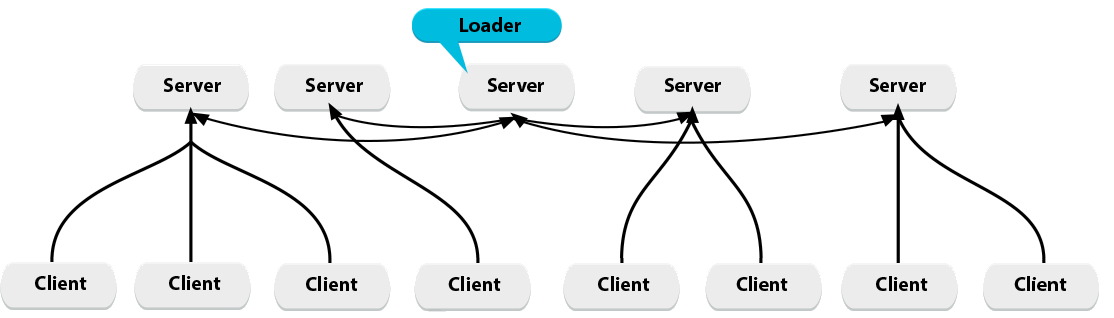
\includegraphics[width=0.9\textwidth]{imagem/arquitetura}
	\caption{Distribuição do Zookeeper}
\end{figure}

A arquitetura do Apache ZooKeeper é fundamental o funcionamento como um serviço de coordenação distribuída confiável. Composta por vários componentes que desempenham papéis específicos na manutenção da consistência e na coordenação de operações em sistemas distribuídos. Vejamos uma descrição mais detalhada da arquitetura do ZooKeeper: \vspace{-1em}
\begin{itemize}
	\item Servidores ZooKeeper:
	\begin{itemize}
		\item Núcleo do sistema. Responsáveis por armazenar e manter os dados compartilhados.
		\item Um conjunto de servidores ZooKeeper forma um \textbf{quórum}, que é um grupo de servidores que cooperam para garantir a disponibilidade e confiabilidade.
		\item No mínimo, ZooKeeper requer um quórum de três servidores para funcionar corretamente. Isso permite tolerância a falhas e eleição dos líderes.
	\end{itemize}
    \item Clientes ZooKeeper:
	\begin{itemize}
		\item Entidades que interagem com os servidores ZooKeeper para realizar operações de leitura e escrita nos dados compartilhados.
        \item Os clientes se conectam a qualquer servidor ZooKeeper no \textbf{quórum} e, em seguida, o sistema gerencia a coordenação entre eles.
	\end{itemize}
    \item Znodes:
	\begin{itemize}
		\item Os dados em ZooKeeper são organizados em uma estrutura de árvore hierárquica chamada \textbf{znodes}.
        \item Cada znode pode conter um pequeno pedaço de dados, semelhante a um arquivo, e é identificado por um caminho único na árvore.
        \item Znodes podem ser usados para armazenar configurações, informações de estado, bloqueios distribuídos e outros dados compartilhados.
	\end{itemize}
    \item Watches:
	\begin{itemize}
		\item Os clientes ZooKeeper podem registrar \textit{watches} em \textbf{znodes}. Isso permite que recebam notificações quando ocorrem alterações nos dados que estão observando.
        \item As notificações de watches são assíncronas e permitem que os clientes reajam a eventos de forma eficiente.
	\end{itemize}
    \item Sessões de Clientes:
	\begin{itemize}
		\item Quando um cliente se conecta a um servidor ZooKeeper, cria uma sessão.
        \item As sessões são usadas para rastrear a conexão entre o cliente e servidor, bem como para manter a consistência nas operações do cliente.
        \item Se um cliente perder sua conexão com o servidor, pode reconectar-se usando sua sessão anterior.
	\end{itemize}
    \item Eleição de Líder:
	\begin{itemize}
		\item ZooKeeper usa um mecanismo de eleição para determinar qual dos servidores em um \textbf{quórum} atuará como líder.
        \item O líder é responsável por coordenar as operações e garantir a consistência dos dados.
        \item Os outros servidores atuam como seguidores e replicam os dados do líder.
	\end{itemize}
\end{itemize}

Essa arquitetura é projetada para ser altamente disponível, tolerante a falhas e consistente. Fornece um serviço de coordenação confiável para sistemas distribuídos, garantindo que várias operações aconteçam de maneira ordenada e consistente. Isso é particularmente útil em ambientes de Big Data, sistemas de mensagens, bancos de dados distribuídos e outros cenários onde a coordenação e consistência são cruciais.

ZooKeeper possui um modelo de dados semelhante a um sistema de arquivos, denominado "Znode". Assim como um sistema de arquivos possui diretórios, os Znodes também são diretórios e podem ter dados associados a eles. O Znode pode ser referenciado por meio de um caminho absoluto separado por barras. Cada servidor no conjunto (ensemble) armazena a hierarquia de Znodes na memória, o que torna a resposta rápida e escalável. Cada servidor mantém um registro de transações que registra cada solicitação de "escrita" no disco. Antes de enviar a resposta ao cliente, a transação deve ser sincronizada em todos os servidores, tornando-a crítica em termos de desempenho. 

Embora pareça uma arquitetura baseada em sistema de arquivos, é aconselhável não usá-la desta forma. Deve ser usado para o armazenamento de pequenas quantidades de dados, para que seja confiável, rápido, escalável, disponível e esteja em coordenação com aplicativos distribuídos.

\subsection{Criar o contêiner Docker}
A forma mais simples para obtermos o Zookeeper é através de um contêiner no Docker. E ainda colhemos o benefício adicional de não termos absolutamente nada deixando sujeira em nosso sistema operacional ou áreas de memória.

Baixar a imagem oficial do Zookeeper: \\
\codigo{\$ docker pull zookeeper}

Criar o contêiner do Zookeeper: \\
\codigo{\$ docker run -d -p 2181:2181 -p 8080:8080 --init --name meu-zookeeper zookeeper}

Essa imagem possui o Zookeeper com uma configuração inicial, podemos ver isso com o comando: \\
\codigo{\$ docker logs meu-zookeeper}

Também está disponível uma página de visualização de comandos, através de respostas em formato JSon em: \\
\url{http://localhost:8080/commands}

\subsection{No contêiner do Zookeeper}
Entrar no contêiner do Zookeeper: \\
\codigo{\$ docker exec -it meu-zookeeper bash}

Ao entrar no contêiner estamos na pasta principal do Zookeeper, retornamos para a raiz: \\
\codigo{\# cd ..}

E entramos na pasta de configuração: \\
\codigo{\# cd conf/}

Nesta vemos o arquivo \textbf{zoo.cfg}: \\
\codigo{\# cat zoo.cfg}

Retornamos a pasta de comandos: \\
\codigo{\# cd ../apache-zookeeper-3.7.0-bin/bin}

\subsection{Comandos do Zookeeper}
Caso o servidor já não fosse iniciado no contêiner por padrão, podemos iniciá-lo com o comando: \\
\codigo{\# ./zkServer.sh start} ou \\
\codigo{\# ./zkServer.sh start-foreground}

Como já está iniciado, podemos ver seu estado: \\
\codigo{\# ./zkServer.sh status}

Mesmo caso acontece com o cliente que já está iniciado, caso contrário usaríamos o comando: \\
\codigo{\# ./zkCli.sh -server Slave1:2181}

Entramos no cliente com o comando: \\
\codigo{\# ./zkCli.sh}

Notamos que nosso cursor mudou para: \\
\codigo{[zk: localhost:2181(CONNECTED) 0]}

Isso mostra que estamos conectados no servidor, evitarei de repetir esse curso para não causar muita confusão, mas observe na medida que inserimos comandos o número será incrementado. Além disso podemos ver essa conexão no navegador através da página: \\
\url{http://localhost:8080/commands/connections}

Criamos um \textbf{ZNode} chamado /teste\_znode: \\
\codigo{create /teste\_znode \aspas{Simples exemplo de dados}}

Verificamos a informação deste com: \\
\codigo{get /teste\_znode}

Ou seu status com: \\
\codigo{stat /teste\_znode}

Que retorna: Simples exemplo de dados. O comando addWatch no Apache ZooKeeper permite aos clientes registrar notificações (\textbf{watches}) em \textbf{znodes} para receber notificações quando ocorrem mudanças nesses znodes. Por padrão seu tipo é PERSISTENT\_RECURSIVE isso está relacionada à natureza dessas notificações e à profundidade com a qual são aplicadas na árvore de \textbf{znodes}: \vspace{-1em}
\begin{itemize}
	\item \textbf{PERSISTENT}: Será acionado quando ocorrerem alterações diretas no \textbf{znode} em que o \textbf{watch} foi registrado. Isso significa que o \textbf{watch} será notificado apenas se houver uma mudança no \textbf{znode} em que foi definido, não nos \textbf{znodes} filhos (descendentes) desse \textbf{znode}.
	\item \textbf{PERSISTENT\_RECURSIVE}: Usado para registrar \textbf{watches} em um \textbf{znode} e em todos os seus \textbf{znodes} filhos, ou seja, em toda a subárvore abaixo do \textbf{znode} onde o \textbf{watch} foi definido. Isso significa que o \textbf{watch} será notificado se houver mudanças no \textbf{znode} em que foi definido, bem como em qualquer \textbf{znode} filho desse \textbf{znode} e assim por diante, recursivamente em toda a hierarquia de \textbf{znodes} abaixo.
\end{itemize}

Esse comando é realizado com: \\
\codigo{addWatch -m PERSISTENT\_RECURSIVE /teste\_znode}

Criamos alguns filhos para este \aspas{/teste\_znode} e mostramos esses usando o comando \textbf{ls}:

\begin{lstlisting}[]
create /teste_znode/filho1 "Um primeiro filho"
create /teste_znode/filho2 "Um segundo filho"
ls /teste_znode
\end{lstlisting}

Podemos eliminar qualquer um desses znodes filhos criados: \\
\codigo{delete /teste\_znode/filho1}

Verificamos as permissões de acesso com: \\
\codigo{getAcl /teste\_znode}

E eliminado o znode e seus filhos com: \\
\codigo{deleteall /teste\_znode/filho1}

Podemos fechar a conexão entre o cliente e servidor com o comando: \\
\codigo{close}

Reabrimos esta conexão com o comando: \\
\codigo{connect}

Verificamos todos os comandos executados: \\
\codigo{history}

Saímos do cliente: \\
\codigo{quit}

Saímos do contêiner: \\
\codigo{\# exit}

E o paramos: \\
\codigo{\# docker stop meu-zookeeper}

\subsection{Eleição no Zookeeper}
Obviamente uma única imagem do Zookeeper não funciona para verificarmos como age a liderança de servidores, pois possui apenas um único servidor, precisamos de ao menos 3 máquinas para isso, porém com o poder do Docker Compose podemos simular em um única máquina este estado.

Criamos um arquivo chamado \textbf{docker-compose.yml}:
\codigo{\$ vim docker-compose.yml}

Com a seguinte codificação:
\begin{lstlisting}[]
version: '3.1'

services:
  zoo1:
    image: zookeeper
    container_name: meu-zoo1
    init: true
    restart: always
    hostname: zoo1
    ports:
      - 2181:2181
      - 8081:8080
    environment:
      ZOO_MY_ID: 1
      ZOO_SERVERS: server.1=zoo1:2888:3888;2181 server.2=zoo2:2888:3888;2181 server.3=zoo3:2888:3888;2181

  zoo2:
    image: zookeeper
    container_name: meu-zoo2
    restart: always
    init: true
    hostname: zoo2
    ports:
      - 2182:2181
      - 8082:8080 
    environment:
      ZOO_MY_ID: 2
      ZOO_SERVERS: server.1=zoo1:2888:3888;2181 server.2=zoo2:2888:3888;2181 server.3=zoo3:2888:3888;2181

  zoo3:
    image: zookeeper
    container_name: meu-zoo3
    restart: always
    init: true
    hostname: zoo3
    ports:
      - 2183:2181
      - 8083:8080
    environment:
      ZOO_MY_ID: 3
      ZOO_SERVERS: server.1=zoo1:2888:3888;2181 server.2=zoo2:2888:3888;2181 server.3=zoo3:2888:3888;2181
\end{lstlisting}

Salvamos o arquivo com ESC e o comando \textbf{:wq}, agora vem a parte divertida, usamos o comando: \\
\codigo{\$ docker-compose up -d}

O que acontece neste momento é criada uma rede (na máquina docker) chamada "zookeeper\_default", que pode ser visualizada com o comando: \\
\codigo{\$ docker network ls}

E três contêineres "meu-zoo1", "meu-zoo2" e "meu-zoo3". Que podem ser visualizados com o comando: \\
\codigo{\$ docker ps}

Na página Web, podemos verificar o líder através das portas: 8081 (para o Zoo1), 8082 (para o Zoo2) e 8083 (para o Zoo3), vamos usar a 8081: \\
\url{http://localhost:8081/commands/leader}

E temos como resposta:
\begin{figure}[H]
	\centering
	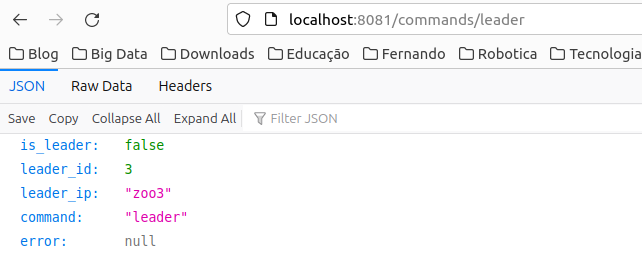
\includegraphics[width=0.6\textwidth]{imagem/lider3}
	\caption{Servidor Líder do Zookeeper}
\end{figure}

Indicando que o líder é o Servidor 3, vamos pará-lo e ver o que acontece: \\
\codigo{\$ docker stop zookeeper\_zoo3\_1}

Ao dar um refresh na página vemos, automaticamente, outro líder foi eleito, assumindo suas funções.
\begin{figure}[H]
	\centering
	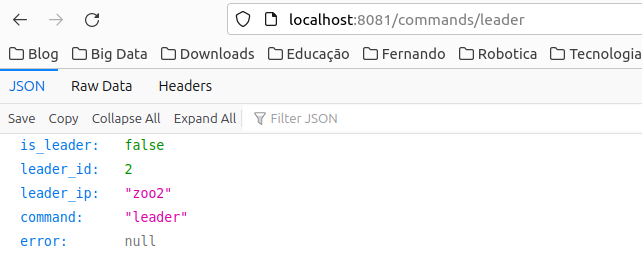
\includegraphics[width=0.6\textwidth]{imagem/lider2}
	\caption{Servidor Líder do Zookeeper}
\end{figure}

Mesmo restaurando o contêiner: \\
\codigo{\$ docker start zookeeper\_zoo3\_1}

Se desejar encerrar todos os contêineres: \\
\codigo{\$ docker-compose stop}

E para iniciá-los: \\
\codigo{\$ docker-compose start}

Ou removê-los: \\
\codigo{\$ docker-compose down}

Ou seja, agora temos o domínio de um ambiente distribuído sem termos que adquirir (ou ter a disposição) várias máquinas para realizarmos testes. Porém o teste mesmo será realizada quando usarmos o \textbf{Apache Kafka} (veja a apostila sobre este).
	
\section{Cliente do Zookeeper com NodeJS}
Vamos usar o \textbf{NodeJS} para exemplificar como podemos verificar o funcionamento do serviço Zookeeper. O primeiro passo é criar uma pasta e inicializá-la com o NodeJS: \\
\codigo{\$ npm init -y}

Precisamos também da biblioteca de comunicação com o Zookeeper: \\
\codigo{\$ npm install node-zookeeper-client}

Criar um arquivo para criar um nó: \\
\codigo{\$ vim meunode.js}

Com o seguinte conteúdo:
\begin{lstlisting}[]
var zookeeper = require('node-zookeeper-client');
var client = zookeeper.createClient('localhost:2181,localhost:2182,localhost:2183');
var path = process.argv[2];
console.log('Estado Atual: %s', client.getState());
var sessionTimeout = client.getSessionTimeout();
console.log('Tempo da Sessão: %s', sessionTimeout)

client.once('connected', function () {
 console.log('Conectado ao servidor.');
 console.log('Estado Atual: %s', client.getState());
 var id = client.getSessionId();
 console.log('Identificação: %s', id.toString('hex'));

 client.create(path, function (error) {
   if (error) {
     console.log('Falhou para criar o node: %s para: %s.', path, error);
   } else {
     console.log('Node: %s is criado corretamente.', path);
   }
   client.close();
 });
});
client.connect();
\end{lstlisting}[]

Salvamos o arquivo pressionando ESC e em seguida \textbf{:wq} e executamos com o seguinte comando: \\
\codigo{\$ node meunode.js /teste}

Criar o arquivo "listarnode.js", com o seguinte conteúdo:
\begin{lstlisting}[]
var zookeeper = require('node-zookeeper-client');
var client = zookeeper.createClient('localhost:2181,localhost:2182,localhost:2183');
var path = process.argv[2];

function listChildren(client, path) {
    client.getChildren(
        path,
        function (event) {
            console.log('Obter o evento watcher: %s', event);
            listChildren(client, path);
        },
        function (error, children, stat) {
            if (error) {
                console.log(
                    'Fallhou para listar o filho de %s para: %s.',
                    path,
                    error
                );
                return;
            }

            console.log('Filhos de %s são: %j.', path, children);
            client.close();
        }
    );
}

client.once('connected', function () {
    console.log('Conectado ao ZooKeeper.');
    listChildren(client, path);
});
client.connect();
\end{lstlisting}[]

Executamos com o seguinte comando: \\
\codigo{\$ node listarnode.js /teste}

Podemos criar os filhos deste node com o comando: \\
\codigo{\$ node meunode.js /teste/teste2}

E assim sucessivamente, criando a estrutura completa que desejamos, veja a documentação completa dessa documentação em: \url{https://www.npmjs.com/package/node-zookeeper-client}

Podemos parar qualquer um dos contêineres de servidores do Zookeeper, que todo o processo continuará sendo executado sem problemas. Outro detalhe interessante é: em qual servidor foram parar esses nodes? Entramos em qualquer um deles: \\
\codigo{\$ docker exec -it meu-zoo1 bash}

Acessamos a pasta de comandos: \\
\codigo{\# cd bin}

Entramos no cliente: \\
\codigo{\# ./zkCli.sh}

E verificamos os nodes para /teste2: \\
\codigo{ls /teste2}

E lá estão nossos nodes filhos: \\
\codigo{[teste1, teste2, teste3, teste4, teste5, teste6]}

Em todos os servidores contém a mesma informação, saímos deste cliente: \\
\codigo{quit}

Saímos do contêiner: \\
\codigo{\# exit}

E podemos repetir esse processo para qualquer servidor que encontramos a mesma informação.

\section{Encerrando a composição}
Encerramos nossa composição com: \\
\codigo{\$ docker-compose stop}

Ou iniciarmos com: \\
\codigo{\$ docker-compose start}

Mas sempre na pasta que se encontra o arquivo \textbf{docker-compose.yml}. Mais fontes de informação podem ser obtidas em diversos sites que apresenta tutoriais completos sobre Zookeeper como a Tutorials Point\cite{tutorialspoint}.

\section{Conclusão}
Aplicativos distribuídos são difíceis de coordenar e trabalhar, uma vez que são muito mais propensos a erros devido ao grande número de máquinas conectadas à rede. Com o envolvimento de várias máquinas, \textit{race conditions} (condições de multi-execução) e deadlocks são problemas comuns na implementação de aplicativos distribuídos. Condições de multi-execução ocorrem quando uma máquina tenta executar duas ou mais operações ao mesmo tempo, e isso pode ser tratado pela propriedade de serialização do ZooKeeper. 

Deadlocks ocorrem quando duas ou mais máquinas tentam acessar o mesmo recurso compartilhado ao mesmo tempo, mais precisamente, tentam acessar os recursos um do outro, o que leva ao travamento do sistema, já que nenhum dos sistemas libera o recurso, mas aguarda o outro sistema liberá-lo. 

A sincronização no ZooKeeper ajuda a resolver os deadlocks. Outro grande problema com aplicativos distribuídos pode ser a falha parcial de processos, o que pode levar à inconsistência dos dados. O ZooKeeper lida com isso por meio da atomicidade, o que significa que ou todo o processo será concluído ou nada persistirá após uma falha. Portanto, o ZooKeeper é uma parte importante do Hadoop que cuida dessas questões pequenas, porém importantes, para que os desenvolvedores possam se concentrar mais na funcionalidade do aplicativo.

Sou um entusiasta do mundo \textbf{Open Source} e novas tecnologias. Qual a diferença entre Livre e Open Source? \underline{Livre} significa que esta apostila é gratuita e pode ser compartilhada a vontade. \underline{Open Source} além de livre todos os arquivos que permitem a geração desta (chamados de arquivos fontes) devem ser disponibilizados para que qualquer pessoa possa modificar ao seu prazer, gerar novas, complementar ou fazer o que quiser. Os fontes da apostila (que foi produzida com o LaTex) está disponibilizado no GitHub \cite{github}. Veja ainda outros artigos que publico sobre tecnologia através do meu Blog Oficial \cite{fernandoanselmo}.

%--------------------------------------------------------------------------
% REFERÊNCIAS
%--------------------------------------------------------------------------
\begin{thebibliography}{4}
	\bibitem{zookeeperoficial} 
	Página do Apache Zookeeper \\
	\url{https://zookeeper.apache.org/}

	\bibitem{tutorialspoint} 
	Tutorials Point sobre Zookeeper \\
	\url{https://www.tutorialspoint.com/zookeeper/index.htm}	
	
		\bibitem{fernandoanselmo} 
	Fernando Anselmo - Blog Oficial de Tecnologia \\
	\url{http://www.fernandoanselmo.blogspot.com.br/}
	
	\bibitem{publicacao} 
	Encontre essa e outras publicações em \\
	\url{https://cetrex.academia.edu/FernandoAnselmo}
	
	\bibitem{github} 
	Repositório para os fontes da apostila \\
	\url{https://github.com/fernandoans/publicacoes}
\end{thebibliography}

\end{document}